\documentclass[border=1mm]{standalone}
\usepackage{tikz}
\usetikzlibrary{shadows,arrows.meta,positioning,calc,patterns, shapes}
\definecolor{darkgreen}{RGB}{27,114,30}

\begin{document}
  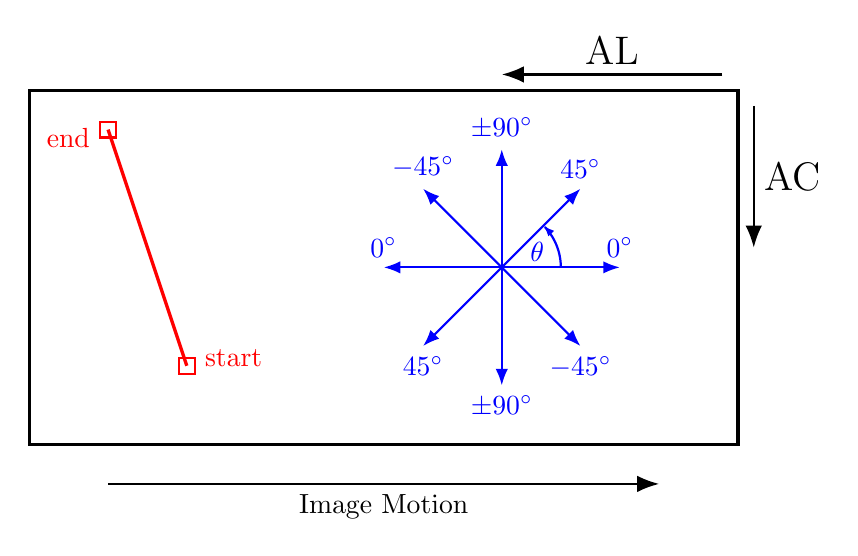
\begin{tikzpicture}[scale=1]

     \draw[very thick] (0,0) rectangle (9,4.5); % The CCD
     % arrows showing AL and AC
     \draw[thick,-{Latex[length=8pt]}] (8.8,4.7) to node [above]{\Large AL} (6,4.7) ;
     \draw[thick,-{Latex[length=8pt]}] (9.2,4.3) to node [right]{\Large AC} (9.2,2.5);
    
     % some cosmic, indicating the start and end
     \draw[very thick,red] (1,4) -- (2,1);
     \draw[thick,red] (1.1,4.1) rectangle (0.9,3.9)  node [above,left]  {end};
     \draw[thick,red] (1.9,0.9) rectangle (2.1,1.1)  node [below,right] {start};
     % a NESW type thing showing what theta is
     \draw[thick,blue,-{Latex[length=6pt]}]  (6,2.25) -- (6,  3.75) %N
          node [above] {$\pm 90^{\circ}$};
     \draw[thick,blue,-{Latex[length=6pt]}]  (6,2.25) -- (7,  3.25) %NE
          node [above] {$45^{\circ}$};
     \draw[thick,blue,-{Latex[length=6pt]}]  (6,2.25) -- (7.5,2.25) %E
          node [above] {$0^{\circ}$};
     \draw[thick,blue,-{Latex[length=6pt]}]  (6,2.25) -- (7,  1.25) %SE
          node [below] {$-45^{\circ}$};
     \draw[thick,blue,-{Latex[length=6pt]}]  (6,2.25) -- (6,  0.75) %S
          node [below] {$\pm 90^{\circ}$};
     \draw[thick,blue,-{Latex[length=6pt]}]  (6,2.25) -- (5,  1.25) %SW
          node [below] {$45^{\circ}$};
     \draw[thick,blue,-{Latex[length=6pt]}]  (6,2.25) -- (4.5,2.25) %W
          node [above] {$0^{\circ}$};
     \draw[thick,blue,-{Latex[length=6pt]}]  (6,2.25) -- (5,  3.25) %NW
          node [above] {$-45^{\circ}$};

    % circle segment
          \draw [blue,thick,domain=0:45,-{Latex[length=4pt]}] plot ({6+0.75*cos(\x)},{2.25+0.75*sin(\x)});
          \draw [blue] (6.45,2.45) node {$\theta$};

     \draw[thick,-{Latex[length=8pt]}] (1,-.5) to node [below]{Image Motion} (8,-.5);
  \end{tikzpicture}
\end{document}
